\documentclass[11pt,letterpaper]{article}

\usepackage[margin=1in]{geometry}
\usepackage{enumitem}
\usepackage{hyperref}
\usepackage{amsmath}
\usepackage{amssymb}
\usepackage{booktabs}
\usepackage{float}
\usepackage{tikz}
\usetikzlibrary{decorations.pathmorphing, decorations.pathreplacing, calc, arrows.meta}

\title{16.07 Dynamics Problem Set 4}
\author{Due Wednesday, October 21}
\date{}

% vector / matrix shorthands
\newcommand{\bw}{\boldsymbol{\omega}}
\newcommand{\bwd}{\boldsymbol{\omega}_d}
\newcommand{\bh}{\mathbf{h}}
% left superscript = frame in which components are expressed
\newcommand{\Bw}{{}^{B}\boldsymbol{\omega}}
\newcommand{\Bwd}{{}^{B}\boldsymbol{\omega}_d}
\newcommand{\Nwd}{{}^{N}\boldsymbol{\omega}_d}
\newcommand{\Bh}{{}^{B}\mathbf{h}}
\newcommand{\Bhd}{{}^{B}\mathbf{h}_d}
\newcommand{\Nh}{{}^{N}\mathbf{h}}
\newcommand{\Nhd}{{}^{N}\mathbf{h}_d}
\newcommand{\Nht}{{}^{N}\mathbf{h}_{\text{tot}}}
\newcommand{\Bht}{{}^{B}\mathbf{h}_{\text{tot}}}
\newcommand{\bJ}{\mathbf{J}}
\newcommand{\bQ}{\mathbf{Q}}
\newcommand{\bx}{\mathbf{x}}
\newcommand{\btau}{\boldsymbol{\tau}}

\begin{document}

\maketitle

\section*{Rigid Body with a Kane Damper}

\begin{figure}[h]
\centering
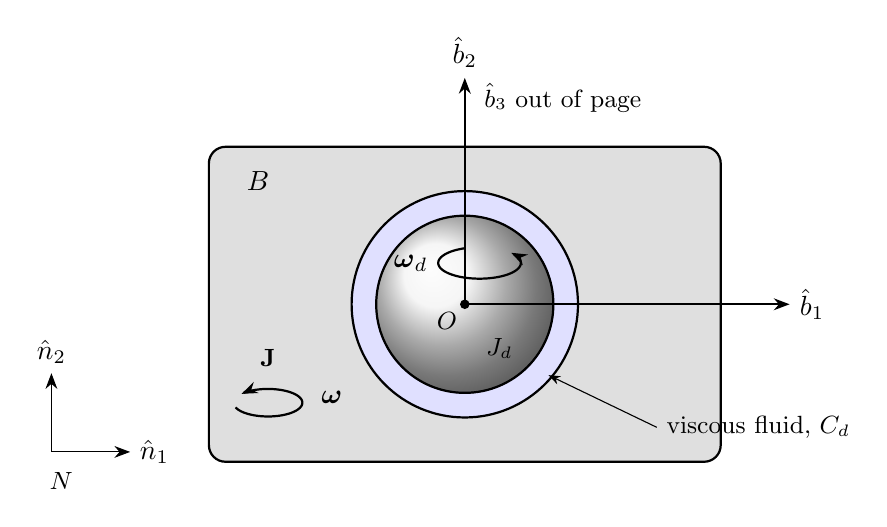
\begin{tikzpicture}[scale=1.25]
    % --- Rigid body (outer shell) ---
    \filldraw[fill=gray!25, draw=black, thick, rounded corners=6pt] (-2.6,-1.6) rectangle (2.6,1.6);
    \node at (-2.1,1.25) {$B$};

    % --- Spherical cavity filled with viscous fluid ---
    \filldraw[fill=blue!12, draw=black, thick] (0,0) circle (1.15);

    % --- Damper sphere ---
    \shade[ball color=gray!10, draw=black] (0,0) circle (0.9);
    \draw[thick] (0,0) circle (0.9);

    % --- Fluid label ---
    \draw[-{Stealth[length=1.5mm]}] (1.95,-1.25) -- (0.85,-0.72);
    \node[anchor=west, font=\small] at (1.95,-1.25) {viscous fluid, $C_d$};

    % --- Damper label and spin ---
    \node[font=\small] at (0.35,-0.45) {$J_d$};
    \draw[-{Stealth[length=2mm]}, thick] plot[domain=110:400, samples=60, variable=\t]
        ({0.42*cos(\t)+0.15},{0.16*sin(\t)+0.42});
    \node at (-0.55,0.42) {$\boldsymbol{\omega}_d$};

    % --- Body frame axes at the shared center of mass O ---
    \filldraw (0,0) circle (1.2pt);
    \node[below left, font=\small] at (0.02,0.02) {$O$};
    \draw[-{Stealth[length=2mm]}, thick] (0,0) -- (3.3,0) node[right] {$\hat b_1$};
    \draw[-{Stealth[length=2mm]}, thick] (0,0) -- (0,2.3) node[above] {$\hat b_2$};
    \node[font=\small, anchor=west] at (0.1,2.1) {$\hat b_3$ out of page};

    % --- Body angular velocity ---
    \draw[-{Stealth[length=2mm]}, thick] plot[domain=200:500, samples=60, variable=\t]
        ({0.35*cos(\t)-2.0},{0.14*sin(\t)-1.0});
    \node at (-1.35,-0.95) {$\boldsymbol{\omega}$};
    \node[font=\small] at (-2.0,-0.55) {$\mathbf{J}$};

    % --- Inertial frame (fixed) ---
    \begin{scope}[shift={(-4.2,-1.5)}]
        \draw[-{Stealth[length=2mm]}] (0,0) -- (0.8,0) node[right] {$\hat n_1$};
        \draw[-{Stealth[length=2mm]}] (0,0) -- (0,0.8) node[above] {$\hat n_2$};
        \node[font=\small] at (0.1,-0.3) {$N$};
    \end{scope}
\end{tikzpicture}
\caption{A rigid body $B$ with a Kane damper: a uniform sphere of moment of inertia $J_d$ spinning freely inside a spherical, fluid-filled cavity. The centers of the cavity and the sphere coincide with the center of mass $O$ of the whole system. The body frame $B$ (unit vectors $\hat b_1, \hat b_2, \hat b_3$) is fixed to the body and aligned with its principal axes; $N$ is an inertial frame. Drawing not to scale.}
\label{fig:kane}
\end{figure}

\noindent A \emph{Kane damper} is a useful simple model of energy dissipation in spinning bodies. It consists of a uniform sphere that is free to rotate inside a slightly larger spherical cavity in the body. The thin gap between the sphere and the cavity wall is filled with a viscous fluid. When the sphere spins at the same rate as the body, nothing happens. When they spin at different rates, the fluid drags the sphere toward the body's motion and the body toward the sphere's motion, dissipating energy as heat.

In this problem set, you'll derive the coupled equations of motion for a rigid body with a Kane damper, then simulate them to see how energy dissipation determines the body's final spin. We'll use the following notation and assumptions throughout:
\begin{itemize}
    \item $N$ is an inertial frame and $B$ is the body frame, with origin at the system center of mass $O$ and axes along the body's principal axes.
    \item $\bJ$ is the inertia matrix of the body about $O$, expressed in $B$. It is constant in $B$.
    \item The damper is a uniform sphere centered at $O$ with scalar moment of inertia $J_d$ about any axis through its center, so its inertia matrix is $J_d\mathbf{I}_{3\times3}$ in \emph{any} frame.
    \item $\bw$ and $\bwd$ are the angular velocities of the body and the damper relative to $N$. A left superscript denotes the frame in which a vector's components are expressed (e.g., $\Bw$), and $\bQ$ is the rotation matrix that maps $B$-frame components to $N$-frame components, ${}^{N}\mathbf{v} = \bQ\,{}^{B}\mathbf{v}$.
    \item The only torques acting are the internal viscous torques between the body and the damper. There are no external torques.
\end{itemize}

\section{Deriving Equations of Motion}

\begin{enumerate}[label=(\alph*)]
    \item \textbf{Angular momenta:} Write the angular momentum of the body, $\Nh$, and of the damper, $\Nhd$, in inertial $N$-frame components. Then write the same vectors in $B$-frame components, $\Bh$ and $\Bhd$, in terms of $\bJ$, $J_d$, $\Bw$, $\Bwd$, and $\bQ$.

    \item \textbf{Transport theorem:} The rate of change of angular momentum \emph{as seen in the inertial frame}, ${}^{N}\dot\bh$, equals the applied torque. However, it is much more convenient to work with components in the body frame, where $\bJ$ is constant. Use the velocity transport theorem to write ${}^{N}\dot\bh$ and ${}^{N}\dot\bh_d$ in terms of $\bQ$, $\Bw$, $\Bwd$, and their time derivatives. Be careful with $\bh_d$: the frame we're differentiating in rotates at $\bw$, not $\bwd$.

    \item \textbf{Damper torques:} We'll model the viscous fluid as a linear damper. The torque applied by the fluid to the body is
    \[
    {}^{B}\btau = C_d\left(\Bwd - \Bw\right),
    \]
    where $C_d > 0$ is the damping coefficient. By Newton's 3rd law, an equal and opposite torque $-{}^{B}\btau$ is applied to the damper. Explain in a sentence why this torque acts to bring the body and damper into co-rotation. Then combine your results from part (b) to derive two coupled vector ODEs for ${}^{B}\dot\bw$ and ${}^{B}\dot\bw_d$.

    \item \textbf{Angular momentum conservation:} Add your two equations from part (c) to show that the total angular momentum $\bh_{\text{tot}} = \bh + \bh_d$ is conserved in $N$, i.e., $\Nht$ is constant. What happened to the damper torques?

    \item \textbf{Energy dissipation:} Write the total kinetic energy $T$ of the system. Using your equations of motion, show that
    \[
    \dot T = -C_d\,\left\lVert \Bwd - \Bw \right\rVert^2 \le 0 .
    \]
    \emph{Hint:} $\mathbf{a}\cdot(\mathbf{a}\times\mathbf{b}) = 0$ for any vectors $\mathbf{a}$ and $\mathbf{b}$.

    \item \textbf{Final state:} Energy keeps decreasing as long as $\bwd \neq \bw$, but $\lVert\bh_{\text{tot}}\rVert$ is fixed. Show that, once the energy stops changing, the body must be spinning about one of its principal axes with the damper locked in co-rotation. For a given $\lVert\bh_{\text{tot}}\rVert$, find the kinetic energy of pure spin about principal axis $i$ in terms of $\lVert\bh_{\text{tot}}\rVert$, the principal moment $J_i$, and $J_d$. About which axis is the energy lowest? Predict what the body's final motion will be.
\end{enumerate}

\section{Simulation}

We'll now simulate the full nonlinear dynamics, including the body's attitude. We'll represent attitude with the rotation matrix $\bQ$, which maps $B$-frame components of a vector to $N$-frame components, ${}^{N}\mathbf{v} = \bQ\,{}^{B}\mathbf{v}$.

\begin{enumerate}[label=(\alph*)]
    \item \textbf{Attitude kinematics:} The rotation matrix evolves according to
    \[
    \dot\bQ = \bQ\,S(\Bw),
    \]
    where $S(\cdot)$ is the skew-symmetric cross-product matrix. Verify that $\dot\bQ$ is \emph{tangent} to the set of rotation matrices, i.e., that if $\bQ^T\bQ = \mathbf{I}$, this equation implies $\dot\bQ^T\bQ + \bQ^T\dot\bQ = \mathbf{0}$, so $\bQ^T\bQ$ stays constant.

    \item \textbf{First-order ODE:} Define the 15-dimensional state vector
    \[
    \bx = \begin{bmatrix} \operatorname{vec}(\bQ) \\ \Bw \\ \Bwd \end{bmatrix},
    \]
    where $\operatorname{vec}(\bQ)$ stacks the columns of $\bQ$ into a $9\times1$ vector. Combine your results from Section~1(c) and part (a) to write the full dynamics as a first-order vector ODE $\dot\bx = \mathbf{f}(\bx)$. Implement $\mathbf{f}$ as a function in MATLAB or Python. \emph{Note:} MATLAB's \texttt{reshape} stacks columns by default; in NumPy, use \texttt{reshape(..., order='F')}.

    \item \textbf{Simulate:} We'll use the T-shaped body from Problem Set 3, with the damper added at its center of mass. Its principal inertia matrix (in CGS units) is
    \[
    \bJ = \operatorname{diag}\left(30.03,\ 43.10,\ 69.09\right)\times10^{3}~\text{g\,cm}^2 ,
    \]
    so $\hat b_1$ is the minor axis, $\hat b_2$ the intermediate axis, and $\hat b_3$ the major axis. Use $J_d = 3000$~g\,cm$^2$ and $C_d = 2000$~g\,cm$^2$/s. Using \texttt{ode45} (MATLAB) or \texttt{scipy.integrate.solve\_ivp} (Python) with relative and absolute tolerances of $10^{-8}$, run three simulations for $t\in[0, 900]$~s, one for each principal axis $k = 1, 2, 3$, with initial conditions
    \[
    \bQ(0) = \mathbf{I}, \qquad
    \Bw(0) = \Omega\,{}^{B}\hat b_k + \boldsymbol{\epsilon}, \qquad
    \Bwd(0) = \Bw(0) + \boldsymbol{\epsilon},
    \]
    where $\Omega = 2$~rad/s and $\boldsymbol\epsilon = \epsilon\,[1\;\,1\;\,1]^T$ with $\epsilon = 10^{-3}$~rad/s is a small perturbation.

    \item \textbf{Momentum and energy:} For each run, plot the following versus time:
    \begin{itemize}
        \item The components of the total angular momentum in the inertial frame, $\Nht = \bQ\left(\bJ\,\Bw + J_d\,\Bwd\right)$, and its magnitude $\lVert\bh_{\text{tot}}\rVert$.
        \item The components of $\Bw$.
        \item The total kinetic energy $T$.
    \end{itemize}
    Each run has a different $\lVert\bh_{\text{tot}}\rVert$, so to compare them on the same footing, plot the normalized energy $2T/\lVert\bh_{\text{tot}}\rVert^2$ for all three runs on a single set of axes. Mark the values corresponding to pure spin about each principal axis from Section~1(f) with horizontal lines. Show that all three runs settle into the global energy minimum: major-axis spin. Describe what happens along the way in the minor-axis and intermediate-axis runs. Why does the major-axis run barely change?

    \item \textbf{Orthogonality of $\bQ$:} A valid rotation matrix must satisfy $\bQ^T\bQ = \mathbf{I}$ and $\det\bQ = +1$. For each run, plot $\lVert\bQ^T\bQ - \mathbf{I}\rVert_F$ (the Frobenius norm) and $\lvert\det\bQ - 1\rvert$ versus time on a log scale. Then repeat one run using the integrator's default tolerances and plot the same quantities.
    \begin{itemize}
        \item Even though part (a) showed that the exact dynamics preserve $\bQ^T\bQ = \mathbf{I}$, the numerical solution does not. Why not?
        \item Does the drift in $\bQ$ affect the computed trajectories of $\Bw$ and $\Bwd$? Does it affect your computed $\Nht$? Explain using the structure of $\mathbf{f}(\bx)$.
        \item Suggest one way to keep $\bQ$ a valid rotation matrix during a long simulation. (You don't need to implement it.)
    \end{itemize}
\end{enumerate}

\end{document}
